\documentclass[a4paper, 12pt, final]{article}

\usepackage[utf8]{inputenc}
\usepackage[francais]{babel}
\usepackage[french]{varioref}
\usepackage{layout} 
\usepackage{listings} 
\usepackage[comma,authoryear]{natbib}
\usepackage{graphicx}

\title{ ELE 470 - Kesako ? \\ Description of the project }

\author{ Laïla Atrmouh }

\date{Tuesday 2 October 2012}

\begin{document}

\maketitle  
   
\rule[0.5ex]{\textwidth}{0.1mm}

\section{Introduction}  
\emph{Kesako?} is a new kind of audioguide for museums and other expositions. The purpose of the project is to get informations about artworks by scanning QR Code. Indeed, each QR Code is linked to a painting, a photography, or more generally an artwork. 

\section{Functionalities}
With this application, a user can :
\begin{itemize}
\item Scan a QRCode to get more informations about an artwork
\item See the last 5 scanned artworks
\end {itemize}

If I have time, I will develop these extra functionalities :
\begin{itemize}
\item Audio description of the artwork (that can be triggered by the user)
\item Rating system (the user will be able to rate the artwork) 
\item Translation in several languages
\end{itemize}

\section {Methods}
\subsection{What is QR Code ?}
QRCode is the trademark for a type of barcode which consists of black pixels arranged in a square pattern on a white background. The advantages of using QRCode are :
\begin {itemize}
\item open-source technology
\item big community
\item free to use
\item fast to read
\end{itemize}  
There is a library ZXing, which allow the reading of QR Codes ( http://code.google.com/p/zxing/ ).  

 \subsection{Where are the informations about the artworks ?}
The informations about the artworks will be stored in an XML file, which will be read at the launch of the application. XML is better to use in order to keep the application the more generic as possible. Indeed, XML is a very widespread technology, each museum can feed the application with its own file. The structure of the XML file would be the following: 
\begin{lstlisting}
<artwork>
	<qrcode>URL Generated by the QRCode</qrcode>
	<title>Title of the artwork</title>
	<desc>Description of the artwork</desc>
</artwork> 
\end{lstlisting} 
As you can see on the models section below, we also show a picture of the artwork. In order to have a small XML file, we can read the media files (photo, audio description) using the url generated by the QRCode. 

\section{Organization}
The project will be cut into three steps :
\begin{itemize}
\item Reading of QR Code
\item Reading of the XML file
\item Development of the functionalities (filling the view with the information associated with the scanned QRCode …)
\end{itemize}

\section{Models} 
These interfaces are not fixed, but the two screens give a general idea of the design of the future app.\\ 
\begin{figure}[!h] %on ouvre l'environnement figure
\centering
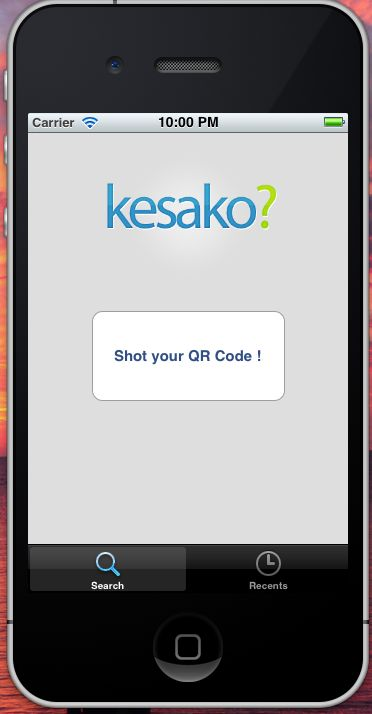
\includegraphics[width=4cm]{1.jpg} %ou image.png, .jpeg etc.
\caption{Scanning of the QRCode using the iPhone's camera} %la légende
\label{api} %l'étiquette pour faire référence à cette image
\end{figure} %on ferme l'environnement figure 
 
\begin{figure}[!h] %on ouvre l'environnement figure
\centering
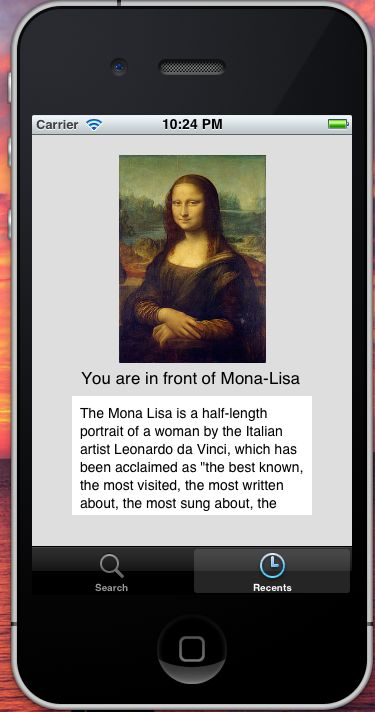
\includegraphics[width=4cm]{2.jpg} %ou image.png, .jpeg etc.
\caption{Second view of the application, informations about the artwork associated with the scanned QRCode} %la légende
\label{api} %l'étiquette pour faire référence à cette image
\end{figure} %on ferme l'environnement figure
 
 
\end{document}
 
